\chapter{FUNDAMENTAÇÃO TEÓRICA}

\section{Exposição do Tema ou Matéria}

\subsection{Hardware dedicado \glspl{gpu}}

No início, a aparência dos gráficos baseados em GPU era um tanto monótona e padronizada devido à falta de programabilidade, mas agora a maioria dos estágios do pipeline gráfico é programável. Infelizmente, observou-se  que o aumento na programabilidade atingiu um limite, e mais liberdade exigiria a capacidade de alterar a própria estrutura do pipeline. Isso, por sua vez, está firmemente enraizado no hardware gráfico específico da GPU e não é facilmente modificado \cite{laine2011high}.

% nao sei oq fazer com o acronimo FIFO
Uma grande parte do trabalho no pipeline gráfico, principalmente a execução de shaders de vertex e fragment, mas também outros estágios programáveis, são realizados pelos núcleos de shader programáveis. Entre esses processos destacam-se \textit{marshaling}(organização de dados)) e \textit{scheduling}(agendamento de operações) de dados. Esses processos incluem gerenciamento de filas FIFO, controle de buffer de quadro na memória on-chip, busca de dados de entrada do shader na memória local antes da execução do shader, acionamento de execuções de shader, execução de operações de rasterização. Realiza cálculos mais triviais, como a construção de equações de borda e plano, rasterização e \textit{clipping} \cite{laine2011high}.

A NVIDIA introduziu o CUDA em 2007. Por meio do CUDA, os núcleos programáveis (shader cores) passaram a ser acessíveis para aplicações de propósito geral \cite{laine2011high}. Tal abordagem possibilita a implementação de algoritmos fora do pipeline gráfico tradicional, ampliando a flexibilidade no desenvolvimento.

A plataforma CUDA apresenta limitações de compatibilidade entre plataformas \cite{song2024parallel}. A AMD criou o HIP, que permite aos desenvolvedores migrarem o código CUDA existente para plataformas AMD \cite{amd_hip_docs}. Como alternativa mais multiplataforma que suporta \glspl{cpu} e outros dispositivos, OpenCL é usado como plataforma de computação paralela \cite{song2024parallel}. Um dispositivo OpenCL pode ser dividido em uma ou mais unidades de computação, e cada uma é composta por um ou mais elementos de processamento (PEs) \cite{song2024parallel}.

As placas gráficas começaram a oferecer cada vez mais funcionalidades programáveis, como sintaxe para shaders, inconsistência entre fornecedores e GPUs móveis que possuem arquitetura baseada em seus requisitos de energia e espaço. O Vulkan resolve esses problemas de compatibilidade por ser projetado para arquiteturas gráficas modernas. Vulkan reduz a sobrecarga de lidar com diversos drivers, permitindo que programadores especifiquem suas intenções por meio de uma \gls{api} \cite{vulkan_tutorial}. Diferentemente das outras plataformas, OpenCL, voltadas à computação de propósito geral, o Vulkan é mais direcionado ao desenvolvimento de aplicações gráficas, como renderização.

\subsection{Primitivas}

Em um sistema de modelagem hierárquica, objetos complexos são construídos a partir da junção de elementos mais básicos organizados em diferentes níveis. Para isso, são necessários elementos que não dependam de outros elementos para serem descritos. Em sistemas hierárquicos, chamamos esses elementos de nível mais baixo de \textit{primitives} (primitivas) \cite{wyvill1995practical}.

No \textit{ray tracing}, as primitivas podem ser: polígonos, objetos geométricos como a esfera ou objetos mais complexos como patches paramétricos \cite{wyvill1995practical}. Na rasterização, é possível usar figuras mais complexas, porém o Vulkan usa apenas pontos, linhas e triângulos, pois são as mais otimizadas. Em especial, os triângulos são amplamente utilizados uma vez que permitem a aproximação de superfícies arbitrárias e complexas \cite{vulkan_docs}.

\subsection{Principais efeitos luminosos}

TODO: reflexão; refração; sombras.

\subsection{\textit{Ray tracing}}

\textit{ray tracing} é uma técnica de renderização gráfica 3D baseada na simulação da propagação da luz real em um cenário virtual tridimensional. O termo pode ser utilizado tanto para se referir a um algoritmo específico, quanto para uma classe de algoritmos que lançam raios através de uma cena. Comparado com a maioria dos outros algoritmos de renderização, o \textit{ray tracing} proporciona um efeito de luz e sombra mais realista. O primeiro algoritmo de \textit{ray tracing} foi proposto por Appel em 1968. Appel criou o \textit{ray casting} \cite{wang2022development}.

O \textit{ray casting} renderiza a cena emitindo um raio primário do ponto de observação ou câmera para cada pixel, encontrando o objeto mais próximo que bloqueia o caminho do raio. Raios adicionais, como raios de sombra, podem ser utilizados para verificar a visibilidade da luz a partir do ponto de interseção \cite{wang2022development}.

\begin{figure}[H]
    \centering
    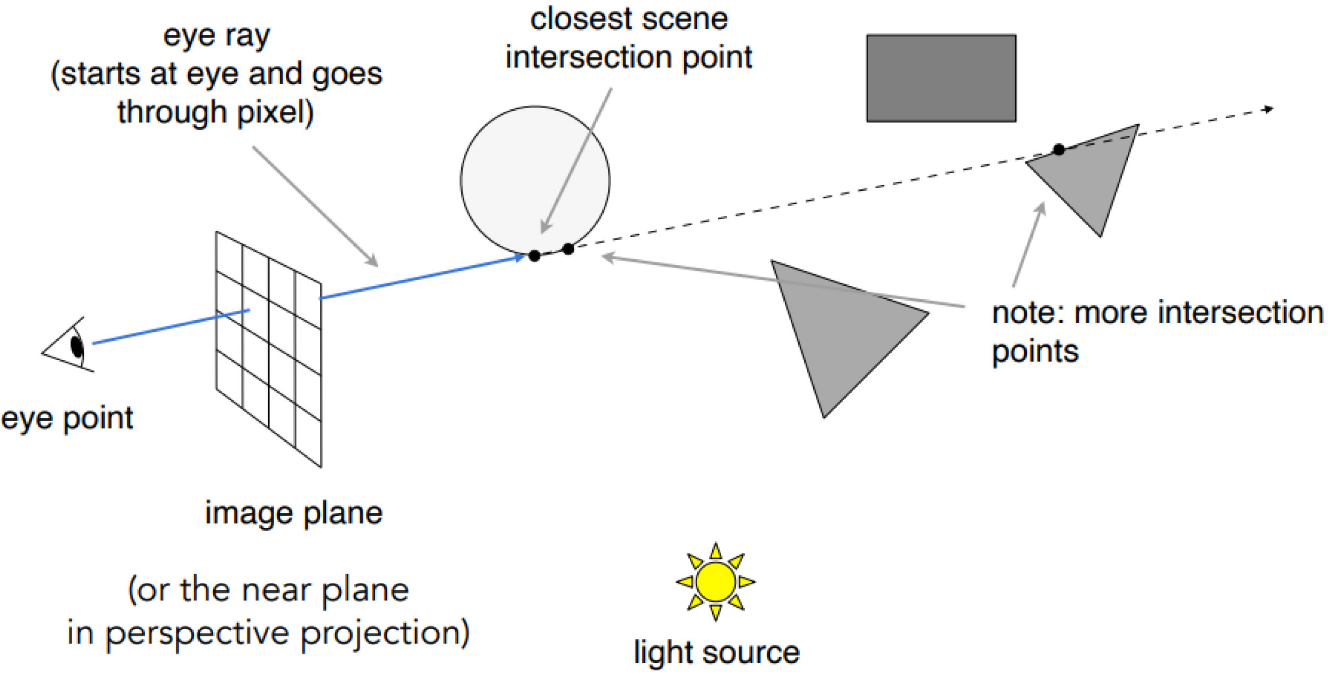
\includegraphics[width=0.7\textwidth]{images/exemploRayCasting.png}
    \caption{Exemplo do funcionamento do \textit{ray casting}. Fonte: \cite{wang2022development}}
    \label{fig:exemplo_ray_casting}
\end{figure}

As faces são orientadas utilizando a regra da mão direita: os vértices são listados em sentido anti-horário quando se olha o objeto do exterior. Para uma face ABC, o vetor normal n=AB*AC aponta para fora. \cite{freud2006fast}.

A equação do raio que parte da câmera é um dos elementos fundamentais do \textit{ray casting}, pois permite determinar o ponto de interseção com os objetos da cena. Essa equação pode ser expressa como \cite{freud2006fast}:

\begin{equation*}
\mathbf{SI} = \beta_p \, \mathbf{SP}, \quad \beta_p \in \mathbb{R}, \; 0 < \beta_p \leq 1
\end{equation*}

Em que:
\begin{itemize}
    \item $S$ representa a posição de origem do raio;
    \item $P$ corresponde ao centro de um pixel no detector;
    \item $\mathbf{SP}$ define a direção do raio;
    \item $I$ é o ponto de interseção do raio e a superfície do objeto;
    \item $\beta_p$ é um parâmetro escalar que determina a posição do ponto de interseção ao longo do raio.
    \item $SI$ é vetor da origem até o ponto de interseção.
\end{itemize}

O Whitted \textit{ray casting}, uma evolução do \textit{ray casting}, foi desenvolvido por Turner Whitted em 1979. Esse algoritmo usa quatro tipos de raios diferentes. O raio da câmera é similar ao \textit{ray casting}. O segundo raio de reflexão simula superfícies refletoras e semirrefletoras. O terceiro raio de refração pode incidir no objeto a partir de um ângulo. O quarto raio de sombra projeta sombra gerada pela fonte de luz e pelo objeto. A superfície nem sempre é perfeitamente refletora, seria necessário modelar um componente difuso, mas modelos de iluminação difusa mais realistas implicam maior custo computacional \cite{wang2022development}.

\begin{figure}[H]
    \centering
    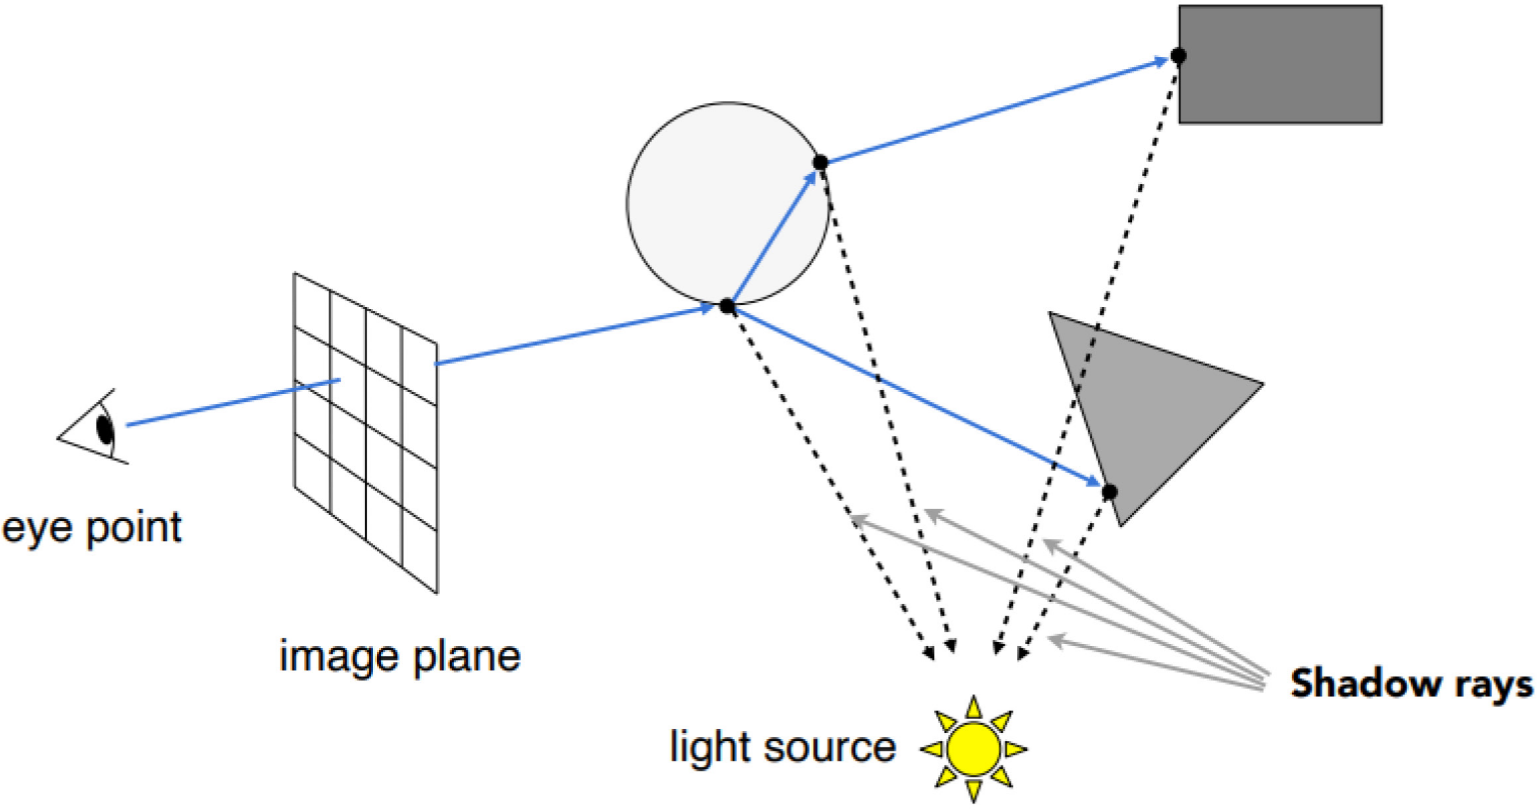
\includegraphics[width=0.7\textwidth]{images/ExemploWhittedRayCasting.png}
    \caption{Exemplo do funcionamento do Whitted \textit{ray casting}. Fonte: \cite{wang2022development}}
    \label{fig:exemplo_whitted_ray_casting}
\end{figure}

\subsection{Rasterização}

A rasterização é uma técnica básica de renderização. Uma tarefa de renderização complexa pode ser dividida em diferentes subtarefas associadas a diferentes objetos. Em seguida, cada objeto é dividido em polígonos projetados na tela. Finalmente, cada pixel coberto pelos polígonos é renderizado \cite{wang2022development}. A rasterização era inicialmente feita por software em CPU, isso é praticamente coisa do passado, pois o hardware gráfico dedicado \gls{gpu} oferece desempenho muito superior e virou o padrão para simulação em tempo real \cite{laine2011high}.

O pipeline de rasterização opera em triângulos projetados e recortados em 2D. O coração do algoritmo de rasterização, \textit{coverage computation} (cálculo de cobertura), determina para todos os pixels (e possivelmente várias subamostras em cada pixel), se eles estão cobertos por um determinado triângulo \cite{davidovivc20123d}.

O teste hierárquico de regiões de pixels para cobertura de triângulos, chamado \textit{binning}, é um fator importante para o desempenho de renderização, pois permite identificar rapidamente áreas da imagem potencialmente cobertas. As regiões podem ser avaliadas em paralelo e hierarquicamente para rapidamente identificar amostras relevantes na tela, reduzindo o número de testes individuais \cite{davidovivc20123d}.

O \textit{coverage test} (teste de cobertura) normalmente usa funções de aresta 2D lineares no espaço da imagem, uma para cada aresta do triângulo, cujo sinal determina qual lado da aresta está dentro do triângulo. Um pixel está dentro do triângulo se todas as três funções de aresta forem positivas em sua localização e, portanto, o cálculo da cobertura se torna uma simples avaliação das três funções de aresta, o que é adequado para arquiteturas paralelas \cite{davidovivc20123d}.

O \textit{clipping} (recorte) à esquerda e à direita pode ser tratado como arestas extras do polígono, representadas por El e Er. Ao considerar esses limites como arestas, o algoritmo de rasterização evita processar partes fora da área visível, parando quando atinge esses limites. O limite superior define onde a renderização começa, e o inferior indica onde ela termina \cite{pineda1988parallel}.

\begin{figure}[H]
    \centering
    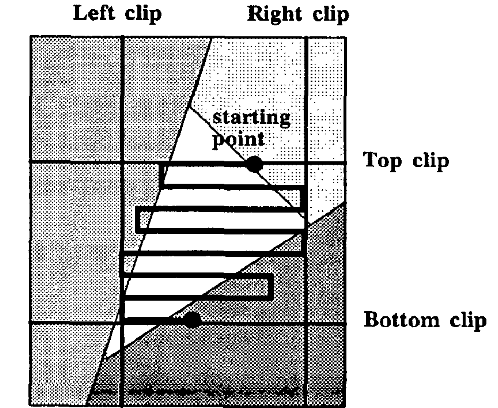
\includegraphics[width=0.7\textwidth]{images/ClippingATriangle.png}
    \caption{Exemplo de triangulo sendo recortado. Fonte: \cite{pineda1988parallel}}
    \label{fig:ClippingATriangle}
\end{figure}

Interpolação, qualquer função linear, u, em um triângulo em 3D, por exemplo, cores ou coordenadas de textura, obedece a u = aX + bY + cZ + d, sendo (X,Y, Z)T um ponto em 3D, e os parâmetros a, b e c podem ser determinados a partir de qualquer conjunto de valores definidos nos vértices. Assumindo o espaço canônico do olho, onde o centro de projeção é a origem, a direção da visão é o eixo z e o campo de visão é de 90 graus, dividir esta equação por Z resulta no conhecido esquema de interpolação correto para perspectiva 2D \cite{davidovivc20123d}.

Testar se uma amostra de pixel é coberta por um triângulo 2D é equivalente a testar se um raio. Um Raio partindo do ponto de vista e passando por esse pixel, intersecta o triângulo. Como exemplo: e é a localização do ponto de vista e o raio passa por d = d0 + xdx + ydy, para coordenadas de pixel (x, y), enquanto p0, p1, p2 são os vértices do triângulo. Podemos formular funções de aresta lineares 3D usando o método de volume com sinal, conhecido como teste de interseção raio-triângulo de Plücker. Na prática, usamos n2 = (p1 - e) x (p0 - p1), que é numericamente mais estável para triângulos pequenos. Definindo a função de aresta 3D correspondente como V2(d) = n2 · d, que é equivalente a calcular o sinal escalonado \cite{davidovivc20123d}.

\begin{figure}[H]
    \centering
    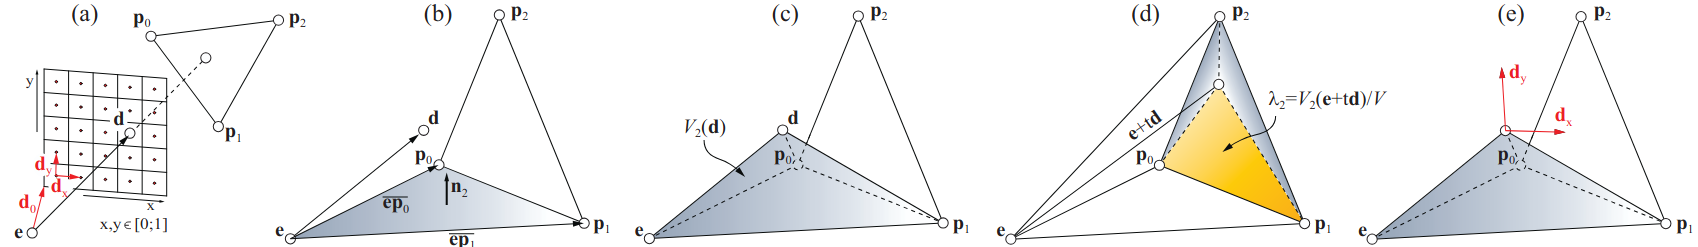
\includegraphics[width=0.7\textwidth]{images/3DEdgeFunction.png}
    \caption{Funções de aresta 3D para um triângulo. \cite{davidovivc20123d}}
    \label{fig:3DEdgeFunction}
\end{figure}

Grande parte do trabalho no pipeline gráfico, principalmente a execução de shaders de \textit{vertex} (vértice) e \textit{fragment} (fragmento), bem como outros estágios programáveis, é realizada pelos núcleos de shader programáveis \cite{laine2011high}.

O \textit{vertex shader} é responsável por decodificar os dados geométricos. Já o \textit{fragment shader} reconstrói o conteúdo da textura ao nível de pixel de saída, por meio da reconstrução do conteúdo da textura via combinação linear \cite{schuster2021compression}.

Durante a rasterização, quando uma primitiva intersecta ou passa à frente de outra, torna-se ambíguo qual delas deve ser visível em cada pixel. O Z-buffer é um algoritmo que resolve a visibilidade ao nível de pixel. O Z-buffer Processa os polígonos, atualiza e armazenando os valores de profundidade de cada pixel durante a conversão da varredura. Não lidam bem com superfícies parcialmente transparentes \cite{greene1993hierarchical}.

\begin{figure}[H]
    \centering
    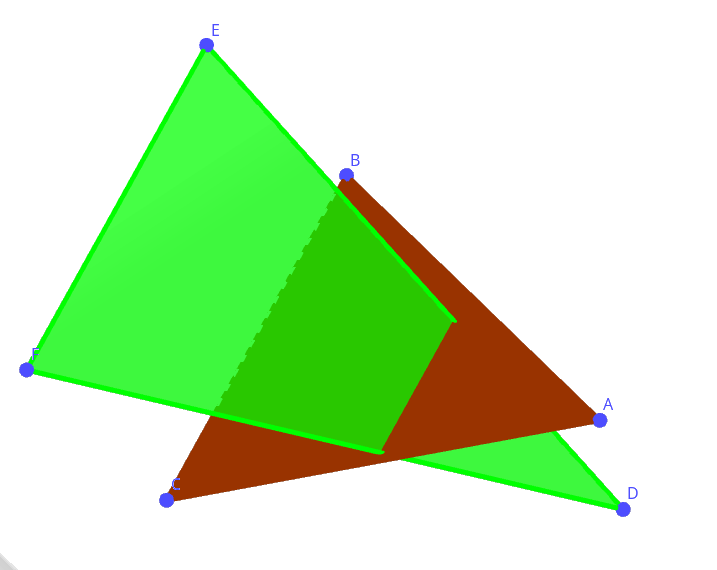
\includegraphics[width=0.7\textwidth]{images/ZBufferCase.png}
    \caption{Caso em que primitivas competem pelo mesmo pixel. Criado pelo autor usando GeoGebra Classic.}
    \label{fig:ZBufferCase}
\end{figure}

A rasterização se tornou a abordagem dominante para aplicações interativas devido aos seus baixos requisitos computacionais iniciais (não requer calculo de ponto flutuante no espaço de imagem 2D), à sua capacidade de ser implementada em hardware e ao desempenho cada vez maior de placas gráficas dedicadas. No entanto, o tratamento de efeitos globais não é nativo e depende de aproximações, como reflexos e sombras \cite{davidovivc20123d}.

\subsection{Abordagem hibrida}

Os dois principais algoritmos usados em computação gráfica para gerar imagens 2D a partir de cenas 3D são a rasterização e o \textit{ray tracing}. A rasterização projeta cada triângulo no plano da imagem e enumera todos os pixels cobertos em 2D, enquanto o \textit{ray tracing} opera em 3D, gerando raios através de cada pixel e encontrando a interseção mais próxima com um triângulo \cite{davidovivc20123d}.

Com a rasterização 3D, as principais diferenças entre as abordagens passam a se concentrar em dois pontos. A travessia da cena, como identificar os objetos relevantes para a cena, usando estruturas e organizações das primitivas. A enumeração de amostras potencialmente cobertas no plano da imagem (binning), que determina quais pixels ou amostras podem ser influenciados por cada primitiva \cite{davidovivc20123d}.

Rasterização e \textit{ray tracing} sao abordagens distintas. Porem, não são técnicas distintas, são pontos extremos de um mesmo espectro contínuo. Sendo assim, diferentes comportamentos podem ser obtidos por meio da ativação ou desativação de determinados componentes, como geração de amostras, binning e testes de oclusão. Permitindo aplicar tanto estratégia de rasterização quanto de ray tracing \cite{davidovivc20123d}.

% ray tracing offline tem q ver isso ai
% verificar se pode ser escrito dessa forma a traducao
Pipeline de renderização híbrida (\textit{Hybrid rendering pipeline}) no qual a rasterização, computação e ray tracing trabalham juntos para possibilitar visuais em tempo real com qualidade próxima à do \textit{ray tracing offline}. A interação de múltiplas etapas gráficas, a utilização das capacidades únicas de cada etapa e a modularização do processo de renderização permitem alcançar vários aspectos visuais de forma otimizada \cite{barre2019hybrid}.

O PICA PICA é um otimo exemplo. PICA PICA é um experimento de traçado de raios em tempo real com agentes de autoaprendizagem em um mundo gerado proceduralmente. O sistema adota um pipeline de renderização híbrida que combina rasterização, shaders de computação e técnicas de \textit{ray tracing} para compor a imagem final. A arquitetura do pipeline é organizada em múltiplas etapas, cada uma responsável por um aspecto específico da renderização, utiliza uma abordagem modular para maximizar eficiência e qualidade visual \cite{barre2019hybrid}.

Para gerar imagens de alta qualidade, seria necessário gerar milhares de amostras por pixel. Mesmo com uma BVH otimizada, algoritmos eficientes de busca e GPUs rápidas, isso não é possível em tempo real atualmente, exceto para as cenas mais simples. As imagens que podem ser geradas com as restrições de desempenho atuais possuem muito ruído. Porém, elas podem ser tratadas com algoritmos de redução de ruído, podendo gerar imagens com apenas um raio por pixel com qualidade próxima a um \textit{ray tracing offline} \cite{akenine2019real}.

\begin{figure}[H]
    \centering
    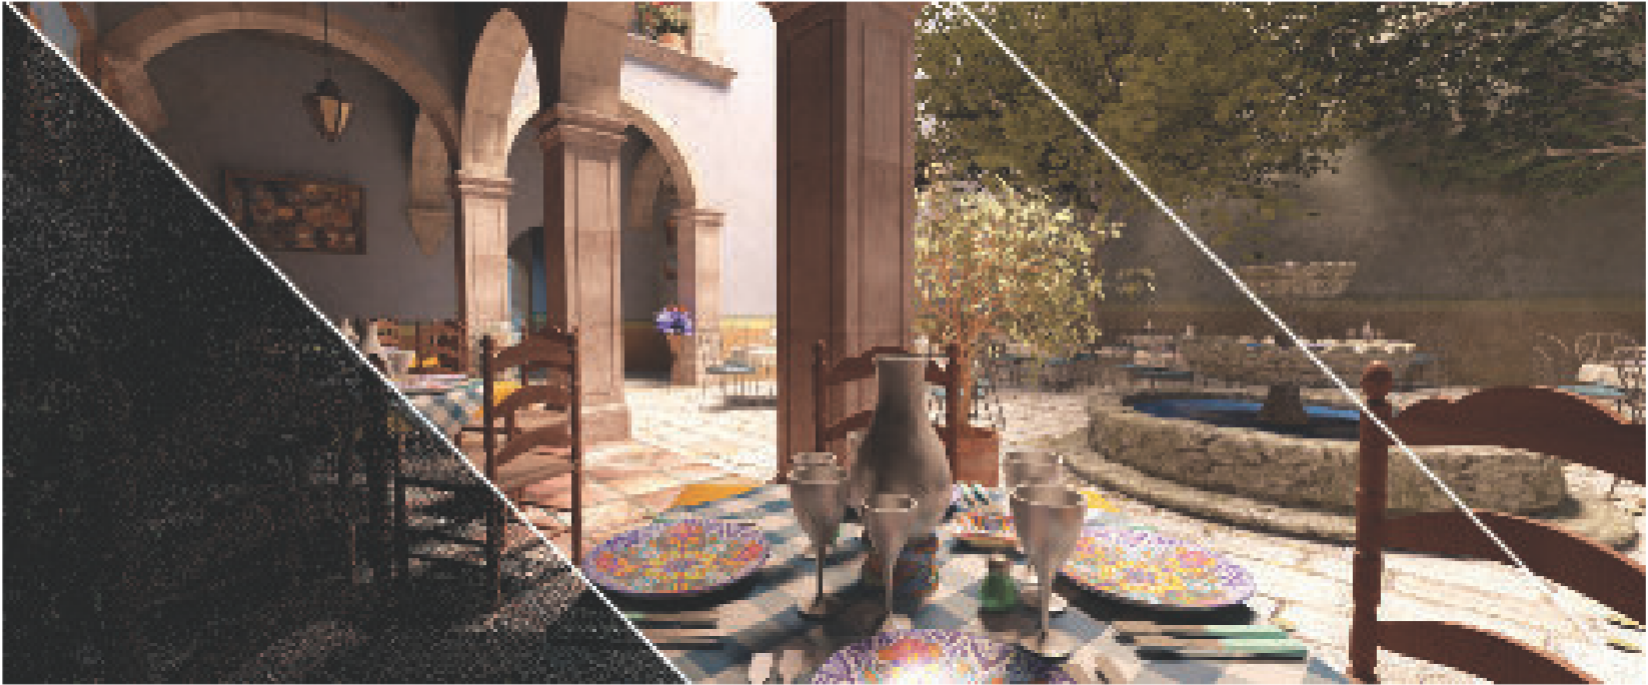
\includegraphics[width=0.7\textwidth]{images/UmaAmostraPorPixelPathTraced.png}
    \caption{Imagem path-traced (esquerda). Imagem suavizada (centro). A qualidade de referência renderizada com 2048 amostras por pixel (direita). Fonte \cite{akenine2019real} cortesia da NVIDIA Corporation.}
    \label{fig:UmaAmostraPorPixelPathTraced}
\end{figure}


O pipeline do PICA PICA se inicia com o \textit{object-space rendering} (renderização no espaço de objetos), trata as estruturas geométricas e coordenadas de textura. Faz o cálculo de transparência e translucidez para raios. Depois, com \textit{global illumination}, calcula oclusão (esse processo é limitado a um número máximo de testes por quadro) \cite{barre2019hybrid}. G-buffer, uma abreviação de \textit{geometric buffers} (buffers geométricos), refere-se a buffers usados para armazenar propriedades de superfície. Cada G-buffer é um alvo de renderização separado. Esse alvo pode ser  mapa de profundidade, buffer normal, buffer de rugosidade, oclusão, cor da textura (albedo), intensidade da luz, intensidade especular e imagem quase final \cite{akenine2019real}.

Usando dados do G-buffer, gera sombras a partir da fonte de luz e remove possíveis ruídos. Pega pontos de partida do G-buffer para lançar raios de reflexão. Calcula a luz direta que vem de uma fonte até o material. Por fim, pós-processamento que adiciona efeitos como \textit{anti-aliasing} (suavização de serrilhado) e desfoque de movimento \cite{barre2019hybrid}.

\subsection{Estruturas de aceleração}

O \textit{ray tracing} vem se tornando cada vez mais importante para aplicações em tempo real. No entanto, exige alto poder computacional e depende de estruturas de dados pré-processadas para alcançar um desempenho em tempo real. Dentre os métodos para melhorar a eficiência do traçado de raios, as estruturas de dados hierárquicas são extremamente importantes e populares \cite{stich2009spatial}.

Representações hierárquicas de objetos tridimensionais são eficientes tanto em tempo quanto em uso de memória. Essas representações tipicamente consistem em árvores cujos ramos representam volumes delimitadores \cite{rubin19803}. A ideia por trás de uma \gls{bvh} é subdividir as primitivas de uma cena em conjuntos possivelmente sobrepostos. Para cada um desses conjuntos, um \gls{bv} é calculado e estes são organizados em uma estrutura de árvore. Os limites de cada nó nesta árvore são escolhidos de forma que ele delimite exatamente todos os nós na subárvore correspondente e cada nó folha delimite exatamente as primitivas contidas \cite{bauszat2010minimal}.

\begin{figure}[H]
    \centering
    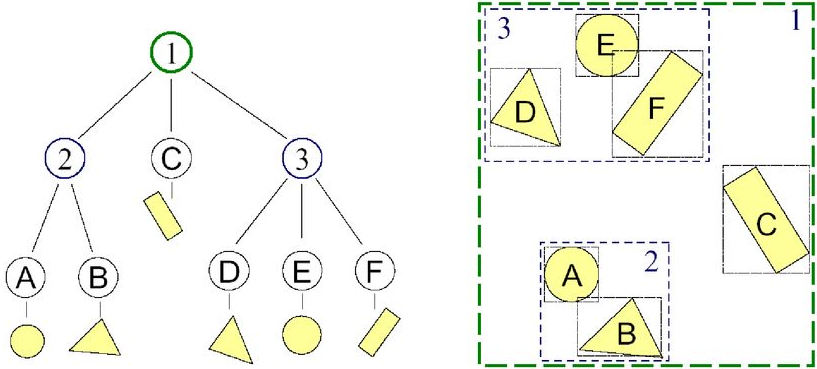
\includegraphics[width=0.7\textwidth]{images/bvhExample.png}
    \caption{Exemplo de \gls{bvh}. Fonte: \cite{singleton_bvh}}
    \label{fig:bvh_example}
\end{figure}

Para encontrar a interseção mais próxima. A travessia de um raio inicia-se no nó raiz e é realizada de forma \textit{top-down} (de cima para baixo). Geralmente, utilizando uma pilha para armazenar nós internos que podem conter a interseção mais próxima. A cada iteração, o nó do topo é removido e o raio é testado contra seu \gls{bv}. Caso haja interseção, seus nós filhos são adicionados à pilha, no caso de nós internos, ou as primitivas são testadas diretamente, no caso de nós folha. Testando as primitivas, armazenamos a distância até a interseção mais próxima encontrada até o momento. Usando essa distância, podemos ignorar os nós que estão mais distantes do que a interseção encontrada anteriormente. A travessia continua até que a pilha esteja vazia. Para um teste de oclusão, quando queremos saber apenas se o ponto está visível ou ocluído, podemos, portanto, usar um \textit{early exit} (saída antecipada) após encontrar a primeira interseção \cite{meister2021survey}.

\begin{figure}[H]
    \centering
    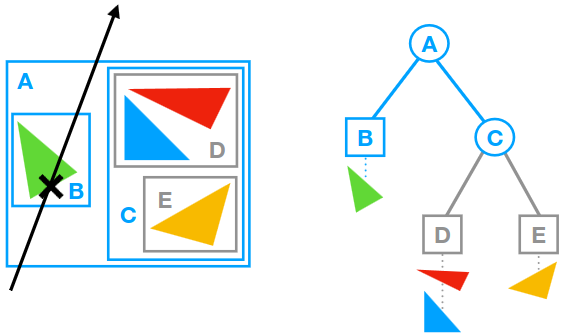
\includegraphics[width=0.7\textwidth]{images/bvhIntersection.png}
    \caption{Exemplo de travessia de \gls{bvh} para encontrar a interseção, descartamos toda a subárvore do nó C, uma vez que o raio não intersecta a caixa delimitadora associada a ela. Fonte: \cite{meister2021survey}}
    \label{fig:bvh_intersection}
\end{figure}

Originalmente, \gls{bvh} utilizava pelo menos seis \textit{bounding slabs} (planos limitantes) para formar um casco fechado ao redor de um objeto. Cada slab corresponde à região compreendida entre dois planos paralelos, que restringem o espaço em uma determinada direção; a interseção desses \textit{slabs} define o volume delimitador \cite{bauszat2010minimal}.

Se esses \textit{slabs} são perpendiculares aos eixos do sistema de coordenadas do mundo, o volume delimitador resultante é denominado \gls{aabb}. Em \glspl{bvh} convencionais, os limites de um \gls{aabb} são representados por seis valores de ponto flutuante, correspondentes às coordenadas mínimas e máximas ao longo de cada eixo cartesiano  \cite{bauszat2010minimal}.

Comparadas a outras abordagens, as \glspl{bvh} têm geralmente os menores requisitos de memória e um \textit{memory footprint} (uso de memória) pré-computável \cite{bauszat2010minimal}. Técnicas híbridas têm sido investigadas minuciosamente nos últimos anos, buscando combinar os benefícios das árvores \glspl{bvh}.

% explicar modelos de BVH utilizados

\subsection{Métricas}

% explicar isso tudo

% build time
% traversal time
% overhead time
% frame time
% latência por frame
% memory footprint total
% memory bandwidth usage
% ocupação de CUDA cores
% warp divergence
% cache efficiency
% consumo energético por frame
% uso da CPU
% uso de memória RAM

% apresentar os modelos q serao usados no trabalho

%
%--------- FIM DESENVOLVIMENTO------------
%